%%
%% ACM SIGSPATIAL '26 SHORT PAPER (4 pp incl. refs) — WJ-native distillation.
%% Condensed, distillation-first. Figures: TikZ pipeline + dim/recall/QPS plot.
%% [RS:] notes flag the few open items (pipeline tweak, held-out baseline re-eval).
%%
\documentclass[sigconf]{acmart}
\usepackage[utf8]{inputenc}
\usepackage{newunicodechar}
\newunicodechar{∼}{\textasciitilde}
\AtBeginDocument{\providecommand\BibTeX{{Bib\TeX}}}

\setcopyright{acmlicensed}
\copyrightyear{2026}\acmYear{2026}\acmDOI{XXXXXXX.XXXXXXX}
\acmConference[SIGSPATIAL '26]{34th ACM SIGSPATIAL}{November 2026}{Atlanta, GA}
\acmISBN{978-1-4503-XXXX-X/2026/11}

\usepackage{amsmath}
\usepackage{booktabs}
\usepackage{graphicx}
\usepackage{tikz}
\usetikzlibrary{positioning,arrows.meta}
\graphicspath{{./}{../figures/}}
\usepackage{pifont}
\usepackage{enumitem}
\newcommand{\cmark}{\ding{51}}\newcommand{\xmark}{\ding{55}}
\newcommand{\rs}[1]{\textcolor{green!55!black}{[RS: #1]}}
\newcommand{\ba}[1]{\textcolor{orange}{[BA: #1]}}

\begin{document}

% Title — method is DISTILLATION (not an autoencoder). Alternatives:
%  (B) Aligning the Objective with the Metric: WJ-Native Distillation for Polygon Retrieval
%  (C) Learning WJ-Preserving Embeddings by Metric Distillation
\title{Weighted-Jaccard-Native Distillation for Compact Polygon
Similarity Search under Extreme Area Variation}

\author{Ruban Sampath}
\affiliation{\institution{Univ. of Texas at San Antonio}\city{San Antonio}\country{USA}}
\email{ruban.s@utsa.edu}
\author{Buddhi Ashan M. K.}
\affiliation{\institution{Univ. of Texas at San Antonio}\city{San Antonio}\country{USA}}
\email{buddhiashan.mallikakankanamalage@utsa.edu}
\author{Sushil K. Prasad}
\affiliation{\institution{Univ. of Texas at San Antonio}\city{San Antonio}\country{USA}}
\email{sushil.prasad@utsa.edu}
\renewcommand{\shortauthors}{Sampath et al.}

\begin{abstract}
Similarity search over polygonal datasets asks which polygons have similar \emph{shape}
(area-weighted overlap, independent of location), and Weighted Jaccard (WJ) is the
standard metric for it. The state-of-the-art ShapeToVec encodes each polygon with a
quad-tree-based non-uniform grid that handles extreme area variation, then indexes the
result with a Hierarchical Navigable Small World (HNSW) graph; however, its high
dimensionality imposes a heavy memory and query-throughput cost. We first trained a
simplex-constrained encoder with a WJ-native triplet loss, false-negative filtering, and
decoder reconstruction: $36\times$ smaller 512-dimensional vectors that, on a 10k subset
of the Parks dataset, reach Recall@50 $=0.858$ at 10{,}903 QPS ($78\times$ faster than
brute-force Improved Consistent Weighted Sampling, ICWS) and Recall@10 $>0.996$ after
exact-WJ reranking. On a larger benchmark, however, this and other ranking-style
objectives no longer beat an untrained random projection: they optimize local separation
rather than the global WJ ranking recall depends on, and the loss even damages the very
layer it is deployed from. We close this gap with \emph{WJ-native distillation}:
regressing the embedding's WJ directly onto the true WJ, aligning the training
objective with the retrieval metric and yielding a single Matryoshka encoder deployable
at any dimension. This is, to our knowledge, the first learned WJ embedding to surpass
random projection on both the near- and wide-net recall--throughput frontiers: on a 50K
benchmark it reaches Recall@500 $=0.924$ ($0.976$ after reranking) at just 256
dimensions ($72\times$ compression), beating random projection at every dimension while
running several-fold faster.
\end{abstract}

\begin{CCSXML}
<ccs2012>
<concept><concept_id>10002951.10003317.10003347.10003350</concept_id>
<concept_desc>Information systems~Similarity search</concept_desc>
<concept_significance>500</concept_significance></concept>
<concept><concept_id>10002951.10003317.10003318</concept_id>
<concept_desc>Information systems~Nearest-neighbor search</concept_desc>
<concept_significance>500</concept_significance></concept>
<concept><concept_id>10010147.10010257.10010293.10010294</concept_id>
<concept_desc>Computing methodologies~Neural networks</concept_desc>
<concept_significance>300</concept_significance></concept>
</ccs2012>
\end{CCSXML}
\ccsdesc[500]{Information systems~Similarity search}
\ccsdesc[500]{Information systems~Nearest-neighbor search}
\ccsdesc[300]{Computing methodologies~Neural networks}
\keywords{polygon similarity search, weighted Jaccard, autoencoder, metric distillation,
approximate nearest neighbor, probability simplex}
\received{June 2026}
\maketitle

%% ---------------- 1. Introduction ----------------
\section{Introduction}
\label{sec:intro}
Finding similar shapes in large polygon datasets is a fundamental geospatial
operation, for deduplication, conflation, and map integration. We study
polygons from the SpatialHadoop GIS benchmark's~\cite{eldawy15} Parks collection
(\S\ref{sec:exp}); water-body and sports collections from the same benchmark are a
natural extension (\S5). Quantifying
shape overlap calls for an area-aware metric; Weighted Jaccard (WJ),
\begin{equation}
  WJ(\mathbf{a},\mathbf{b}) = \frac{\sum_i \min(a_i,b_i)}{\sum_i \max(a_i,b_i)},
  \quad \mathbf{a},\mathbf{b} \ge \mathbf{0},
  \label{eq:wj}
\end{equation}
is the standard choice, where $\mathbf{a},\mathbf{b}\in\mathbb{R}^D_{\ge0}$ are two
polygons' vector encodings over a shared partition of $D$ spatial cells and $a_i$ is
polygon $\mathbf{a}$'s area-weighted occupancy of cell $i$. The core difficulty is
\emph{extreme area variability}: polygon areas span several orders of magnitude
(e.g.\ a neighbourhood park versus a national forest), and a single uniform grid
cannot serve both regimes: a grid fine enough to resolve small polygons explodes in
dimension at the scale of large ones, while a grid coarse enough to be tractable
leaves small polygons occupying only a handful of cells, collapsing their shape
information into near-empty vectors. ShapeToVec~\cite{shape2vec} resolves this with an adaptive
\emph{quadtree} grid that recursively subdivides space where polygon detail is
concentrated, encoding each polygon as a high-dimensional probability-simplex
vector (tens of thousands of dimensions, varying with grid resolution) whose WJ
preserves overlap across scales. Indexed with HNSW~\cite{hnsw20} under a \emph{custom}
Weighted Jaccard distance (added by ShapeToVec~\cite{shape2vec} to
NMSLIB~\cite{boytsov13}), it reaches $97\%$ R@50
on up to 1.7M polygons. But such large vectors are costly to store and search;
compressing them while preserving WJ structure is our goal.

Existing tools do not fit. WJ sketches (ICWS~\cite{ioffe10},
ProbMinHash~\cite{probminhash20}, PolyMinHash~\cite{polyminhash25}) output integer
codes needing brute-force or LSH-band search; learned hashing and metric
learning~\cite{hashsurvey14,deephashsurvey22} target Hamming or cosine spaces;
none produce WJ-compatible embeddings. Our contributions are as follows:
\begin{enumerate}[leftmargin=1.2em,itemsep=1pt,topsep=1pt]
  \item A \textbf{WJ-native simplex encoder}: a similarity-sensitive encoder whose
    ReLU\,+\,$\ell_1$ output lies on the probability simplex, compressing
    high-dimensional ShapeToVec encodings into compact embeddings indexable directly
    under WJ, without post-processing.
  \item A \textbf{shape-similarity distillation loss}: WJ-native distillation
    regresses the embedding's WJ onto the true (shape-overlap) WJ, making the training
    objective the retrieval metric: the first learned WJ embedding to beat an
    untrained random projection (\S\ref{sec:exp}).
  \item \textbf{Matryoshka deployment}: a single trained model serves every
    embedding width $\{256, 512, \dots,4096\}$, giving the full recall--throughput frontier from one round of training; 256-d dominates.
\end{enumerate}

%% ---------------- 2. Related Work ----------------
\section{Related Work}
\label{sec:related}
\textbf{ShapeToVec and its gap.} ShapeToVec~\cite{shape2vec} is the state of the art
for WJ polygon retrieval: its adaptive quadtree grid encodes each polygon as a
high-dimensional floating-point simplex vector, and a custom Weighted Jaccard
distance it adds to NMSLIB~\cite{boytsov13} lets HNSW index these vectors directly,
reaching $97\%$ R@50 (versus $67\%$ for its binary bit-vector variant). That accuracy,
however, rests on tens of thousands of dimensions: ShapeToVec itself notes that such
vectors strain HNSW memory as datasets grow, and that generic compression
(e.g.\ product quantization) shrinks the footprint only by \emph{degrading} accuracy.
We fill this gap with a learned, WJ-native compression, up to $72\times$ smaller,
while preserving (indeed improving) WJ retrieval.
WJ \emph{sketching} (ICWS~\cite{ioffe10}, ProbMinHash~\cite{probminhash20},
PolyMinHash~\cite{polyminhash25}) gives unbiased estimators but integer codes
incompatible with float-vector approximate-nearest-neighbor (ANN) indexes. Learned
hashing~\cite{hashsurvey14,deephashsurvey22} and Matryoshka representation
learning~\cite{matryoshka22} target Hamming/cosine spaces and degrade on the WJ
simplex (Table~\ref{tab:results}); NMF~\cite{nmf99} gives simplex factors but
optimises reconstruction, not retrieval. Knowledge distillation~\cite{hinton15}
transfers a teacher's outputs to a student; we adapt it to a \emph{metric},
distilling exact WJ into a compact simplex embedding; none of the above target
WJ as the native metric.

\textbf{Ranking objectives vs.\ value regression.} Learning-to-rank losses such as
RankNet~\cite{burges05} and ListNet~\cite{cao07} are a further alternative: rather
than pushing a single hardest negative below a margin (\S\ref{sec:contrastive}),
they optimise pairwise or listwise order directly and could plausibly avoid the
margin loss's collapse at scale. We do not rule this out, but choose direct value
regression (\S\ref{sec:distill}) for a different reason: it makes the training
objective identical to the deployed metric, not merely correlated with the
neighbour ordering it induces, so the compact embedding's WJ is meaningful on its
own (e.g.\ for thresholding), not just for ranking a fixed candidate set. A
head-to-head comparison against listwise ranking losses is left to future work.

%% ---------------- 3. Method ----------------
\section{Method}
Given ShapeToVec vectors $\mathbf{x}\in\Delta^{D}$ ($D$ in the tens of thousands) and ground-truth
WJ neighbour pairs, we learn $f_\theta:\Delta^{D}\!\to\!\Delta^{d}$ ($d\le512$)
preserving WJ for fast HNSW retrieval (Fig.~\ref{fig:pipeline}).

\begin{figure}[t]\centering
\resizebox{\columnwidth}{!}{%
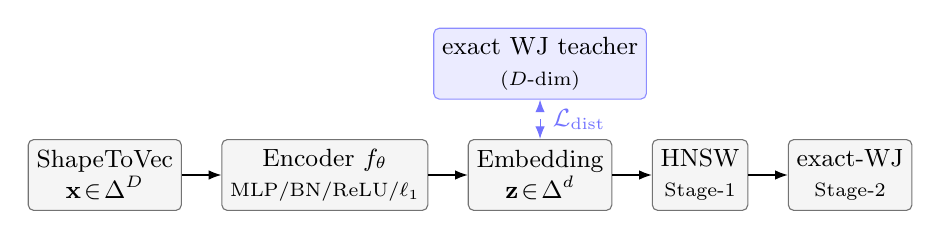
\begin{tikzpicture}[font=\small,>={Latex[length=1.6mm,width=1.2mm]},
  node distance=4.5mm and 5mm,
  box/.style={draw=black!55,rounded corners=2pt,fill=black!4,
              minimum height=9mm,align=center,inner sep=3pt},
  tbox/.style={box,fill=blue!8,draw=blue!45}]
 \node[box] (x) {ShapeToVec\\$\mathbf{x}\!\in\!\Delta^{D}$};
 \node[box,right=of x] (e) {Encoder $f_\theta$\\{\scriptsize MLP/BN/ReLU/$\ell_1$}};
 \node[box,right=of e] (z) {Embedding\\$\mathbf{z}\!\in\!\Delta^{d}$};
 \node[tbox,above=5mm of z] (t) {exact WJ teacher\\{\scriptsize ($D$-dim)}};
 \node[box,right=of z] (h) {HNSW\\{\scriptsize Stage-1}};
 \node[box,right=of h] (r) {exact-WJ\\{\scriptsize Stage-2}};
 \draw[->](x)--(e); \draw[->](e)--(z);
 \draw[<->,dashed,blue!55](z)--node[right=0.4mm]{$\mathcal{L}_{\mathrm{dist}}$}(t);
 \draw[->](z)--(h); \draw[->](h)--(r);
\end{tikzpicture}}
\caption{WJ-native pipeline. The encoder maps a quadtree vector onto the
probability simplex; training distills the exact $D$-dim WJ (teacher) into the
embedding's WJ; retrieval is HNSW Stage-1 then exact-WJ rerank.
}
\label{fig:pipeline}
\end{figure}

\subsection{Encoder Architecture}
\label{sec:embed}
The encoder's core, $h_\theta$, is a two-layer MLP ($D\!\to\!4096\!\to\!4096$,
$\sim$92M parameters); its $4096$-d output is $\ell_1$-normalised
(Eq.~\ref{eq:simplex}, \S\ref{sec:simplex}) and truncated to width $d$ at inference
(Matryoshka, \S\ref{sec:distill}). Three considerations dictate this design, each
driven by the structure of WJ and of the quadtree input rather than by convention.

\noindent\textbf{Why an MLP, not a Transformer or graph encoder.} The neural polygon
encoders common in the literature, boundary Transformers~\cite{mai22}, vertex graph
networks~\cite{polygongnn24}, and set encoders~\cite{deepsets17}, target cosine or
Euclidean output spaces and are ill-suited to WJ retrieval. Two mismatches explain
this. First, \emph{space mismatch}: an encoder trained under an L2 or cosine
objective learns a metric structure that is destroyed when its outputs are forced
onto the WJ simplex via ReLU\,+\,$\ell_1$-normalisation. Second, \emph{loss of
global structure}: sequence- and graph-based encoders aggregate \emph{local}
context (token windows, vertex hops), whereas WJ is a global statistic summed over
all $D$ dimensions that cannot be decomposed into local sub-computations. A plain
MLP trained \emph{natively} in WJ space avoids both.

\noindent\textbf{Global projection.} Accordingly, the first layer is a single dense
projection $\mathbb{R}^{D}\!\to\!\mathbb{R}^{4096}$ that mixes \emph{all} input
dimensions in one matrix multiply, so every pair of quadtree cells can interact and
the cross-dimension co-occurrence statistics WJ depends on are preserved. This
global mixing is why $\sim$75M of the $\sim$92M parameters reside in this first
layer.

\noindent\textbf{BatchNorm before ReLU.} Quadtree rasterisation yields extremely
sparse vectors ($\sim$73\% zeros), so pre-activation responses have near-zero
variance; applying ReLU directly would suppress almost all activations and produce a
degenerate output whose pairwise WJ is too flat to rank candidates. Placing
BatchNorm~\cite{ioffe15bn} \emph{before} each ReLU re-centers and rescales the
activations first, guaranteeing a non-degenerate output distribution.

\subsection{Probability Simplex Output Constraint}
\label{sec:simplex}
WJ (Eq.~\ref{eq:wj}) requires non-negative inputs. We enforce this with a final
simplex projection layer:
\begin{equation}
  f_\theta(\mathbf{x}) = \frac{\mathrm{ReLU}(h_\theta(\mathbf{x}))}
       {\max(\|\mathrm{ReLU}(h_\theta(\mathbf{x}))\|_1,\;\epsilon)} \in \Delta^{d}.
  \label{eq:simplex}
\end{equation}
The sequence BatchNorm~$\to$~ReLU~$\to$~$\ell_1$-normalisation is necessary and
sufficient for WJ compatibility: non-negativity makes the element-wise $\min$/$\max$
in Eq.~\ref{eq:wj} meaningful, and $\ell_1$-normalisation places every embedding on
the probability simplex $\Delta^{d}$ so the $\min$/$\max$ ratio is computed at a
comparable scale regardless of polygon size. Together this makes
$WJ(f_\theta(\mathbf{x}),f_\theta(\mathbf{y}))$ well-defined for any input pair and
enables direct use of nmslib's \texttt{WeightedJaccard} HNSW
space~\cite{shape2vec,boytsov13} with no post-processing.

\subsection{Why contrastive objectives are not enough}
\label{sec:contrastive}
Our first approach was metric learning, which we describe here and show why it
fails, motivating \S\ref{sec:distill}. With anchor--positive pairs and in-batch
cross-WJ $S_{ij}=WJ(f_\theta(\mathbf{a}_i),f_\theta(\mathbf{p}_j))$, a
\emph{false-negative filter} $\mathcal{G}$ masks a query's true neighbours before
mining the hardest negative
$j^\star=\arg\max_{j\neq i,(i,j)\notin\mathcal{G}}S_{ij}$, and a triplet
loss~\cite{schroff15} with margin $m$,
\begin{equation}
  \mathcal{L}_{\mathrm{trip}}=\big[\,WJ(\mathbf{n}_{j^\star},\mathbf{a})
     -WJ(\mathbf{p},\mathbf{a})+m\,\big]_{+},
  \label{eq:triplet}
\end{equation}
separates positives from negatives; a decoder reconstruction term and a
non-saturating InfoNCE~\cite{oord18},
\begin{equation}
  \mathcal{L}_{\mathrm{NCE}}=-\log\frac{\exp(S_{ii}/\tau)}
       {\sum_{j:(i,j)\notin\mathcal{G}}\exp(S_{ij}/\tau)},
  \label{eq:infonce}
\end{equation}
extend the supervised neighbourhood. These are strong at 10k
(Table~\ref{tab:results}) but fail to scale: all optimise the same thing,
pushing positives above negatives, which does not guarantee the global WJ
\emph{ranking} that recall depends on. Their recall collapses to that of an
untrained random projection, and the loss \emph{damages the very layer it is
applied to}, so the deployed output is not the network's best representation
(\S\ref{sec:exp}). This motivates supervising the metric itself, directly, next.

\subsection{WJ-native distillation}
\label{sec:distill}
We align the objective with the metric directly. For a batch of $N$ encodings we
form the true WJ on the original $D$-dim vectors, $T_{ij}=WJ(\mathbf{x}_i,\mathbf{x}_j)$,
and the embedding WJ, $\hat T_{ij}=WJ(f_\theta(\mathbf{x}_i),f_\theta(\mathbf{x}_j))$, and minimise
\begin{equation}
  \mathcal{L}_{\mathrm{dist}}=\frac{1}{N^2}\sum_{i,j}\big(\hat T_{ij}-T_{ij}\big)^2 .
  \label{eq:distill}
\end{equation}
Each batch's $N$ rows are anchors and their top-30 WJ neighbours (mined once per
corpus, \S\ref{sec:contrastive}), so $T$ spans both genuine near-neighbour pairs and
the far more numerous low-similarity cross-pairs a random polygon pair would have:
exactly the full range Eq.~\eqref{eq:distill} needs to regress, since, unlike the
margin losses of \S\ref{sec:contrastive}, it must reproduce similarity
\emph{values}, not just their order, to be interchangeable with exact WJ at query
time. Figure~\ref{fig:batchdist} shows this empirically for one 10k training batch:
the curated anchor--positive pairs concentrate at high similarity (mean
$T{=}0.78$), while the remaining, uncurated cross-pairs are not degenerately
concentrated at zero either (mean $0.19$, median $0.13$; only $10.5\%$ fall below
$0.01$) -- MSE is not spending most of its gradient on trivial near-zero pairs, and
retains the low-similarity signal that lets Eq.~\eqref{eq:distill} distinguish
genuine non-matches from moderate partial overlap.

\begin{figure}[t]\centering
\includegraphics[width=0.85\columnwidth]{fig_batch_wj_dist.png}
\caption{Distribution of the WJ distillation target $T_{ij}$ within one training
batch (10k), split into curated anchor--positive pairs (top-30 neighbours) and the
remaining in-batch cross-pairs. The cross-pairs are broadly spread, not
concentrated at zero.}
\label{fig:batchdist}
\end{figure}

The objective \emph{is} the retrieval metric, so the deployed output is exactly the
optimised quantity: a metric distillation~\cite{hinton15} with exact $D$-dim WJ
as teacher and the compact simplex embedding as student. We apply
Eq.~\eqref{eq:distill} on nested prefixes $\{256, 512, \dots,4096\}$
(Matryoshka~\cite{matryoshka22}, each $\ell_1$-renormalised), so one model truncates
to any width; the smallest %already 
dominates (\S\ref{sec:exp}).

\subsection{Two-stage retrieval}
\label{sec:twostage}
Stage-1 builds an HNSW index ($M{=}20$, $\mathrm{ef}{=}200$)~\cite{hnsw20} under
ShapeToVec's custom Weighted Jaccard distance~\cite{shape2vec} over the $d$-dim
embeddings and retrieves a candidate pool of size $K$ per query; Stage-2 reranks
only that pool by exact WJ on the original $D$-dim vectors (Numba~\cite{lam15}),
recovering near-exact ordering within it. Because Stage-2 can only reorder the pool
Stage-1 hands it, not enlarge it, $K$ is the single knob that trades recall for
speed end to end: a larger $K$ costs more HNSW and rerank time but is more likely to
contain the true top-$k$ neighbours; the compact embedding's job is to make a
\emph{small} $K$ already contain them.

%% ---------------- 4. Experiments ----------------
\section{Experiments}
\label{sec:exp}
We use the publicly released ShapeToVec dataset~\cite{shapetovec-data}: quadtree
encodings and shape-similarity ground truth for the Parks polygons (233{,}773;
sourced from SpatialHadoop~\cite{eldawy15}), at its highest-fidelity resolution
($D{=}18{,}382$ dimensions for the 50K benchmark, ${\sim}18.2$--$18.5$k across
subsets), the finest, costliest-to-index resolution and so the most valuable to
compress. The main benchmark is a 50K set partitioned into a 40k-polygon \emph{corpus}
(the indexed database that queries are searched against) and 10k held-out query
polygons; we also use a 10k subset (8k corpus / 2k queries) for the moderate-scale
study and the full 187k Parks corpus (46{,}754 queries) for a scaling check. At 50k
and 187k, learned methods are \emph{corpus-trained}: trained only on
corpus-internal neighbour pairs, so every query is held out and the numbers measure
generalization to unseen queries; at 10k they are trained on the 2k-query set. Ground
truth is the exact \emph{geometric} (shapely) Jaccard on the polygon geometry, which
the quadtree-vector WJ approximates to within $0.999$ R@500. We report R@$k$ ($k\in\{10,50,500\}$) and QPS (PyTorch~\cite{paszke19},
AdamW~\cite{loshchilov19}, cosine annealing~\cite{loshchilov17}). All runs use an
NVIDIA DGX~A100 (8$\times$ A100-SXM4 80\,GB GPUs, dual 64-core AMD EPYC~7742 CPUs,
2\,TB RAM); QPS is measured on a single GPU. \footnote{Code, trained models, and
evaluation scripts: \url{https://github.com/ruban-ai/polygon-ann-ml-embeddings}.}

\begin{table}[t]\centering
\caption{Stage-1 recall on the 10k subset (no rerank). $\dagger$~brute-force.
\textbf{Bold}~=~best ANN method; $\ddagger$~=~ours.}
\label{tab:results}\setlength{\tabcolsep}{4pt}\small
\begin{tabular}{@{}llrrrr@{}}
\toprule
Method & Dim & R@10 & R@50 & R@500 & QPS \\
\midrule
PCA~\cite{jolliffe02}                   & 512  & 0.432 & 0.553 & 0.789 & 16{,}666 \\
NMF~\cite{nmf99}                        & 512  & 0.638 & 0.727 & 0.942 & 11{,}764 \\
Rand.\ Proj.~\cite{achlioptas03}        & 512  & 0.687 & 0.759 & 0.930 &  9{,}663 \\
ICWS~\cite{ioffe10}$^\dagger$           & 512  & 0.840 & 0.897 & 0.988 &     139 \\
Matryoshka MLP~\cite{matryoshka22}      & 512  & 0.455 & 0.672 & 0.932 & 18{,}647 \\
\addlinespace[2pt]
MLP WJ-triplet$^\ddagger$               & 512  & 0.677 & 0.806 & 0.964 & 10{,}756 \\
InfoNCE--WJ$^\ddagger$                  & 512  & 0.490 & 0.698 & 0.947 &  7{,}160 \\
AE WJ-tri+recon$^\ddagger$              & 512  & 0.711 & 0.858 & 0.977 & 10{,}903 \\
\textbf{WJ-distillation}$^\ddagger$ & \textbf{512} & \textbf{0.844} & \textbf{0.930} & \textbf{0.994} & \textbf{14{,}552} \\
\bottomrule
\end{tabular}
\end{table}

\textbf{Moderate scale (Table~\ref{tab:results}).}
WJ-distillation is the strongest method: R@50 $=0.930$, $+7.2$\,pp over the best
contrastive model and above brute-force ICWS (0.897) at ${>}100\times$ its
throughput. Reranking lifts R@10 above $0.996$ for all variants (not shown).

\textbf{The 50K benchmark (Table~\ref{tab:full50k}).}
On 40k corpus polygons with 10k fully held-out queries, the contrastive methods
collapse to the level of an untrained random projection: triplet and InfoNCE reach
only Stage-1 R@500 $\approx 0.72$, at or below random projection ($0.77$--$0.84$
across dimensions). WJ-distillation, by aligning objective and metric, reaches
R@500 $=0.924$ at 256-d, and after reranking delivers the highest recall at the
highest throughput: R@500 $=0.976$ at 6{,}772 QPS. Even at its best dimension
(4096-d), random projection reaches only $0.972$ reranked, still below
distillation's 256-d $0.976$, and at ${\sim}10\times$ the latency. To our knowledge,
this is the first learned WJ embedding to beat random projection on \emph{both} the
near- and wide-net frontiers.

\textbf{Recall by polygon class (Table~\ref{tab:bucket}).} The paper's motivating
claim is that extreme area variation is the hard case (\S\ref{sec:intro}), so we
break the 50K benchmark's Stage-1 recall down by query-polygon area quartile (Q1 =
smallest 25\% of the 10k held-out queries by encoded area, Q4 = largest) and,
separately, by quadtree-cell count (a shape-complexity proxy; same pattern, omitted
for space). WJ-distillation is essentially flat across the size range (R@50
$0.784$--$0.801$), while random projection degrades sharply on large polygons: R@50
falls from $0.753$ at Q1 to $0.594$ at Q4, a $16$pp gap absent from distillation.
The compact embedding does not merely match random projection on average, as
Table~\ref{tab:full50k} shows; it is uniform across exactly the axis of variation
ShapeToVec was built to handle, where the untrained baseline is not.

\begin{table}[t]\centering
\caption{Stage-1 recall by polygon-area quartile (50K benchmark, 256-d, no rerank).
Q1 = smallest 25\% of held-out queries by encoded area, Q4 = largest.
$\ddagger$~=~ours.}
\label{tab:bucket}\setlength{\tabcolsep}{3pt}\footnotesize
\begin{tabular}{@{}lrrrr@{}}
\toprule
Quartile & Distill R@50$^\ddagger$ & Distill R@500$^\ddagger$ & RP R@50 & RP R@500 \\
\midrule
Q1 (smallest) & 0.792 & 0.933 & 0.753 & 0.854 \\
Q2             & 0.801 & 0.910 & 0.661 & 0.729 \\
Q3             & 0.800 & 0.913 & 0.637 & 0.734 \\
Q4 (largest)   & 0.784 & \textbf{0.942} & 0.594 & 0.776 \\
\bottomrule
\end{tabular}
\end{table}

\textbf{Why contrastive fails (Fig.~\ref{fig:layer}).}
The collapse is due to objective--metric misalignment, not capacity limit. Within a
trained contrastive model, Stage-1 recall \emph{rises} the further a layer sits from
the loss: the deployed output is the \emph{worst} layer (R@500 $0.65$, below random
projection's $0.77$), while an untouched intermediate layer is best ($0.82$). Rank
fidelity mirrors this: the Spearman correlation between embedding-WJ and true-WJ
falls from $0.76$ at that layer to $0.14$ at the output, so the loss harms exactly
the representation it is meant to produce.

\begin{figure}[t]\centering

\includegraphics[width=0.74\columnwidth]{fig_layer_tap.png}
\caption{The contrastive loss damages the layer it is applied to. Within one trained
contrastive model, Stage-1 recall \emph{falls} the closer the layer is to the loss:
the deployed 512-d output is the \emph{worst} layer, below an untrained random
projection, while an untouched intermediate layer is best.}
\label{fig:layer}
\end{figure}

\textbf{The full Parks corpus (Table~\ref{tab:full187}).}
Our WJ-distillation encoder, with identical architecture, loss, and 256-d prefix as on
the 50K benchmark, scales unchanged to the full 187k Parks corpus: trained only on
corpus neighbours and evaluated on \emph{all} 46{,}754 held-out queries, it reaches
Stage-1 R@500 $=0.890$ and $0.966$ after reranking.

\begin{table}[t]\centering
\caption{50K benchmark (40k corpus / 10k held-out queries; geometric-Jaccard GT).
All methods corpus-trained, shown at 256-d. $\ddagger$~=~ours. \textbf{Bold}~=~best.}
\label{tab:full50k}\setlength{\tabcolsep}{3.5pt}\small
\begin{tabular}{@{}llrrrr@{}}
\toprule
Method & $K$ & R@10 & R@50 & R@500 & QPS \\
\midrule
\multicolumn{6}{@{}l@{}}{\textit{Stage 1 — no rerank}}\\[1pt]
Rand.\ Proj.~\cite{achlioptas03}    & --- & 0.616 & 0.659 & 0.766 & 3{,}890 \\
triplet+recon$^\ddagger$            & --- & 0.494 & 0.600 & 0.725 & 3{,}810 \\
InfoNCE--WJ$^\ddagger$              & --- & 0.459 & 0.560 & 0.720 & 7{,}128 \\
\textbf{WJ-distillation}$^\ddagger$ & --- & \textbf{0.692} & \textbf{0.794} & \textbf{0.924} & \textbf{6{,}772} \\
\midrule
\multicolumn{6}{@{}l@{}}{\textit{Stage 2 — exact-WJ rerank}}\\[1pt]
Rand.\ Proj.~\cite{achlioptas03}    & 2000 & 0.994 & 0.995 & 0.955 & 904 \\
triplet+recon$^\ddagger$            & 2000 & 0.994 & 0.994 & 0.859 & 898 \\
InfoNCE--WJ$^\ddagger$              & 2000 & 0.993 & 0.987 & 0.821 & 1{,}345 \\
\textbf{WJ-distillation}$^\ddagger$ & 2000 & \textbf{0.995} & \textbf{0.997} & \textbf{0.976} & \textbf{1{,}253} \\
\bottomrule
\end{tabular}
\end{table}

\begin{table}[t]\centering
\caption{The full 187k Parks corpus: WJ-distillation on \emph{all}
46{,}754 held-out queries (corpus-trained), 256-d prefix.} %$\ddagger$~=~ours.}
\label{tab:full187}\setlength{\tabcolsep}{4pt}\small
\begin{tabular}{@{}lrrrr@{}}
\toprule
Stage & R@10 & R@50 & R@500 & QPS \\
\midrule
Stage-1 (no rerank)        & 0.720 & 0.797 & 0.890 & 2{,}136 \\
\textbf{+ exact-WJ rerank} & \textbf{0.993} & \textbf{0.995} & \textbf{0.966} & 1{,}166 \\
\bottomrule
\end{tabular}
\end{table}

\textbf{A second polygon class: water bodies (Table~\ref{tab:wb50k}).} Every result
so far is on Parks; to test whether WJ-distillation is Parks-specific we build an
identically-scaled benchmark (40k corpus / 10k held-out queries, methodology
matching \S\ref{sec:exp}) on the SpatialHadoop water-body
collection~\cite{eldawy15}, with the same architecture, loss, and 256-d prefix,
no method changes. The gap over random projection is, if anything, larger than on
Parks: Stage-1 R@50 $=0.815$ vs.\ $0.632$ ($+18.3$pp) and R@500 $=0.930$ vs.\
$0.763$ ($+16.7$pp), at higher throughput ($4{,}632$ vs.\ $2{,}652$ QPS). After
reranking, distillation's 256-d reaches R@500 $=0.987$ at $1{,}280$ QPS
($K{=}2000$), versus random projection's best dimension (4096-d) reaching only
$0.971$ at $246$ QPS, the same pattern as the Parks 50K benchmark
(\S\ref{sec:exp}). WJ-native distillation is not tuned to one polygon class.

\begin{table}[t]\centering
\caption{Water-body benchmark (40k corpus / 10k held-out queries; same
methodology as the Parks 50K benchmark), shown at 256-d. $\ddagger$~=~ours.
\textbf{Bold}~=~best.}
\label{tab:wb50k}\setlength{\tabcolsep}{3.5pt}\small
\begin{tabular}{@{}llrrrr@{}}
\toprule
Method & $K$ & R@10 & R@50 & R@500 & QPS \\
\midrule
\multicolumn{6}{@{}l@{}}{\textit{Stage 1 --- no rerank}}\\[1pt]
Rand.\ Proj.~\cite{achlioptas03}    & --- & 0.563 & 0.632 & 0.763 & 2{,}652 \\
\textbf{WJ-distillation}$^\ddagger$ & --- & \textbf{0.722} & \textbf{0.815} & \textbf{0.930} & \textbf{4{,}632} \\
\midrule
\multicolumn{6}{@{}l@{}}{\textit{Stage 2 --- exact-WJ rerank}}\\[1pt]
Rand.\ Proj.~\cite{achlioptas03}    & 2000 & 0.994 & 0.994 & 0.958 & 362 \\
\textbf{WJ-distillation}$^\ddagger$ & 2000 & \textbf{0.995} & \textbf{0.997} & \textbf{0.987} & \textbf{1{,}280} \\
\bottomrule
\end{tabular}
\end{table}

\textbf{Trade-off between dimension and throughput (Fig.~\ref{fig:dim}, Table~\ref{tab:dim}).}
Because the encoder is Matryoshka, one model serves every width. Distillation's
recall is essentially flat from 256 to 4096 (R@500 $0.924\!\to\!0.925$) while QPS
falls ${\sim}7\times$, so 256-d, a $72\times$ compression, is the natural
operating point. Baselines, by contrast, stay below distillation at \emph{every} width.

\begin{figure}[t]\centering

\includegraphics[width=0.86\columnwidth]{fig_dim_distill.png}
\caption{WJ-distillation on the 50K benchmark: Stage-1 recall is flat across
dimension while HNSW throughput rises sharply at small $d$; 256-d is the sweet
spot.}
\label{fig:dim}
\end{figure}

\begin{table}[t]\centering
\caption{50K Stage-1 recall vs.\ dimension (40k corpus, 10k held-out queries).
Distillation is one Matryoshka model truncated per row; baselines shown for
contrast (256\,/\,4096). $\ddagger$~=~ours.}
\label{tab:dim}\setlength{\tabcolsep}{3pt}\footnotesize
\begin{tabular}{@{}lrrrr@{}}
\toprule
Method ($d$) & R@10 & R@50 & R@500 & QPS \\
\midrule
triplet+recon$^\ddagger$ & 0.494\,/\,0.495 & 0.600\,/\,0.601 & 0.725\,/\,0.734 & 3810\,/\,710 \\
InfoNCE$^\ddagger$       & 0.459\,/\,0.464 & 0.560\,/\,0.563 & 0.720\,/\,0.720 & 7128\,/\,1168 \\
Rand.\ Proj.             & 0.616\,/\,0.705 & 0.659\,/\,0.749 & 0.766\,/\,0.841 & 3890\,/\,704 \\
\addlinespace[2pt]
\textbf{Distill} 256$^\ddagger$ & \textbf{0.692} & \textbf{0.794} & \textbf{0.924} & 6{,}772 \\
\textbf{Distill} 512$^\ddagger$ & 0.697 & 0.799 & 0.926 & 3{,}111 \\
\textbf{Distill} 1024$^\ddagger$ & 0.698 & 0.800 & 0.926 & 2{,}258 \\
\textbf{Distill} 2048$^\ddagger$ & 0.697 & 0.799 & 0.926 & 1{,}180 \\
\textbf{Distill} 4096$^\ddagger$ & 0.693 & 0.796 & 0.925 & 967 \\
\bottomrule
\end{tabular}
\end{table}

\textbf{Ablation (Table~\ref{tab:ablation}).} On 10k, the false-negative
filter is essential: adding WJ regression \emph{without} it collapses recall to
R@10 $=0.510$, while with it recall is restored (R@50 $0.808$); decoder
reconstruction then adds $+5.0$\,pp R@50 (to $0.858$).

\begin{table}[t]\centering
\caption{Component ablation (Stage-1, 10k, no rerank). The FN filter and decoder
reconstruction are both required; without filtering, WJ regression collapses.}
\label{tab:ablation}\small\setlength{\tabcolsep}{4pt}
\begin{tabular}{@{}llcrr@{}}
\toprule
Model & FN filter & Aux.\ loss & R@10 & R@50 \\
\midrule
MLP & \xmark & ---           & 0.677 & 0.806 \\
MLP & \cmark & ---           & 0.656 & 0.773 \\
MLP & \xmark & WJ regression & 0.510 & 0.736 \\
MLP & \cmark & WJ regression & 0.669 & 0.808 \\
AE  & ---    & recon.\ only  & 0.665 & 0.745 \\
\textbf{AE} & \cmark & \textbf{triplet+recon} & \textbf{0.711} & \textbf{0.858} \\
\bottomrule
\end{tabular}
\end{table}

%% ---------------- 5. Conclusion ----------------
\section{Conclusion}
We compress ShapeToVec WJ vectors up to $72\times$ with a WJ-native simplex embedding.
Contrastive objectives work at moderate scale but collapse to random-projection level
at 50K, since they optimise separation rather than the WJ ranking recall needs.
WJ-native distillation removes this misalignment: a single Matryoshka encoder beats
random projection at both near- and wide-net recall, confirmed up to 187k polygons.
Future work targets billion-scale corpora and other simplex-embeddable set metrics.

\begin{acks}
Claude (Anthropic) assisted with debugging and manuscript formatting.
\end{acks}

\bibliographystyle{ACM-Reference-Format}
\bibliography{refs}
\end{document}
